\documentclass[11pt]{article}

\usepackage[margin=0.9in]{geometry}
\usepackage{graphicx}
\usepackage{amsmath}
\usepackage{amssymb}
\usepackage{xcolor}
\usepackage{caption}
\usepackage{float}
% placeins is unavailable on this system; with [H] floats are placed in-line, so
% a no-op \FloatBarrier suffices to keep each figure with its paragraph.
\providecommand{\FloatBarrier}{}
\usepackage[colorlinks=true,linkcolor=accent,urlcolor=accent,citecolor=accent]{hyperref}

% --- both figure roots: our solo PNGs + composites, and the raw paper crops ---
\graphicspath{{figures_solo/}{../../references/paper_figures/}}

% --- colours ---
\definecolor{accent}{RGB}{20,90,150}
\definecolor{accentlight}{RGB}{232,240,248}
\definecolor{warn}{RGB}{150,70,20}

% --- section heading styling: a touch of colour ---
\makeatletter
\renewcommand\section{\@startsection{section}{1}{\z@}%
  {-3.0ex \@plus -1ex \@minus -.2ex}%
  {1.8ex \@plus.2ex}%
  {\normalfont\large\bfseries\color{accent}}}
\makeatother

\captionsetup{font=small,labelfont={bf,color=accent}}
\setlength{\parskip}{0.4em}
\setlength{\parindent}{0pt}

\newcommand{\headlinebox}[1]{%
  \begin{center}
  \setlength{\fboxsep}{11pt}%
  \setlength{\fboxrule}{1.1pt}%
  \fcolorbox{accent}{accentlight}{%
    \begin{minipage}{0.93\textwidth}
    #1
    \end{minipage}}%
  \end{center}}

\begin{document}

% ===================== TITLE BLOCK =====================
\begin{center}
{\color{accent}\rule{\textwidth}{1.4pt}}\\[1.0em]
{\LARGE\bfseries Custodial vs.\ Minimal: a 2$\times$2 Comparison\par}
\vspace{0.5em}
{\large One $2\times2$ grid per observable --- \textbf{paper} vs.\ \textbf{ours},
\textbf{no custodial} vs.\ \textbf{custodial}.\par}
\vspace{0.5em}
{\normalsize June 2026\par}
\vspace{0.3em}
{\color{accent}\rule{\textwidth}{1.4pt}}
\end{center}
\vspace{0.6em}

% ===================== INTRODUCTION =====================
\section{The question, and the one-line answer}

\textbf{The question.} Does custodial symmetry
($\mathrm{SU(2)}_L\times\mathrm{SU(2)}_R\times\mathrm{U(1)}_X\times P_{LR}$) move
the floors that our minimal-RS scan actually runs into? For each of three
observables we put four panels on a strict $2\times2$ grid: the published figure
(\textbf{\textcolor{warn}{PAPER}}, left column) beside our fixed-code
reproduction (\textbf{\textcolor{accent}{OURS}}, right column), \emph{without}
custodial (top row) above \emph{with} custodial (bottom row).

\textbf{The one-line answer.} Custodial is an \emph{electroweak} cure, not a
\emph{flavor} cure. It pulls the electroweak floors down --- the oblique $T$
parameter collapses to $\sim0$ and the $Z\,b\bar b$ shifts collapse onto the SM
--- but it leaves the $\varepsilon_K$ wall flat at tens of TeV, because the
binding kaon operator is the color-octet KK-gluon $C_4$, an electroweak singlet
the custodial group cannot touch. This is visible \emph{both} in the literature
and in ours: Blanke's \emph{full} custodial $\Delta F{=}2$ calculation finds the
same $\varepsilon_K$ wall as the minimal anarchic scans.

\headlinebox{%
{\bfseries\color{accent} How to read each grid.}\;
Columns: \textbf{\textcolor{warn}{PAPER}} (cropped published figure) $\mid$
\textbf{\textcolor{accent}{OURS}} (our code).
Rows: \textbf{no custodial} (top) $\mid$ \textbf{custodial} (bottom).
For $\varepsilon_K$ the two OURS panels are deliberately the \emph{same} cloud
(custodial changes nothing); for $S,T,U$ and $Z\to b\bar b$ the bottom-row
trajectory visibly relaxes toward the SM. The detailed provenance, attribution,
and per-paper floor tables live in
\texttt{custodial\_comparison.tex}; this note is just the pictures.
\par}

\textbf{Lane note.} The $\varepsilon_K$ comparison uses our \textbf{anarchic
baseline (lane A)} --- the literature strawman --- so it lines up against
Bauer/Blanke. Production as run (lane B, fit-aligned MFV) is a sharper wall at
$\approx$7~TeV; the FPR/aligned ideal (lane C) is $\approx$2~TeV. Custodial moves
\emph{none} of these flavor lanes; only flavor alignment does.

\FloatBarrier
\clearpage

% ===================== (1) eps_K =====================
\section{(1)\quad $\varepsilon_K$ --- the wall does \emph{not} move}

\begin{figure}[H]
\centering
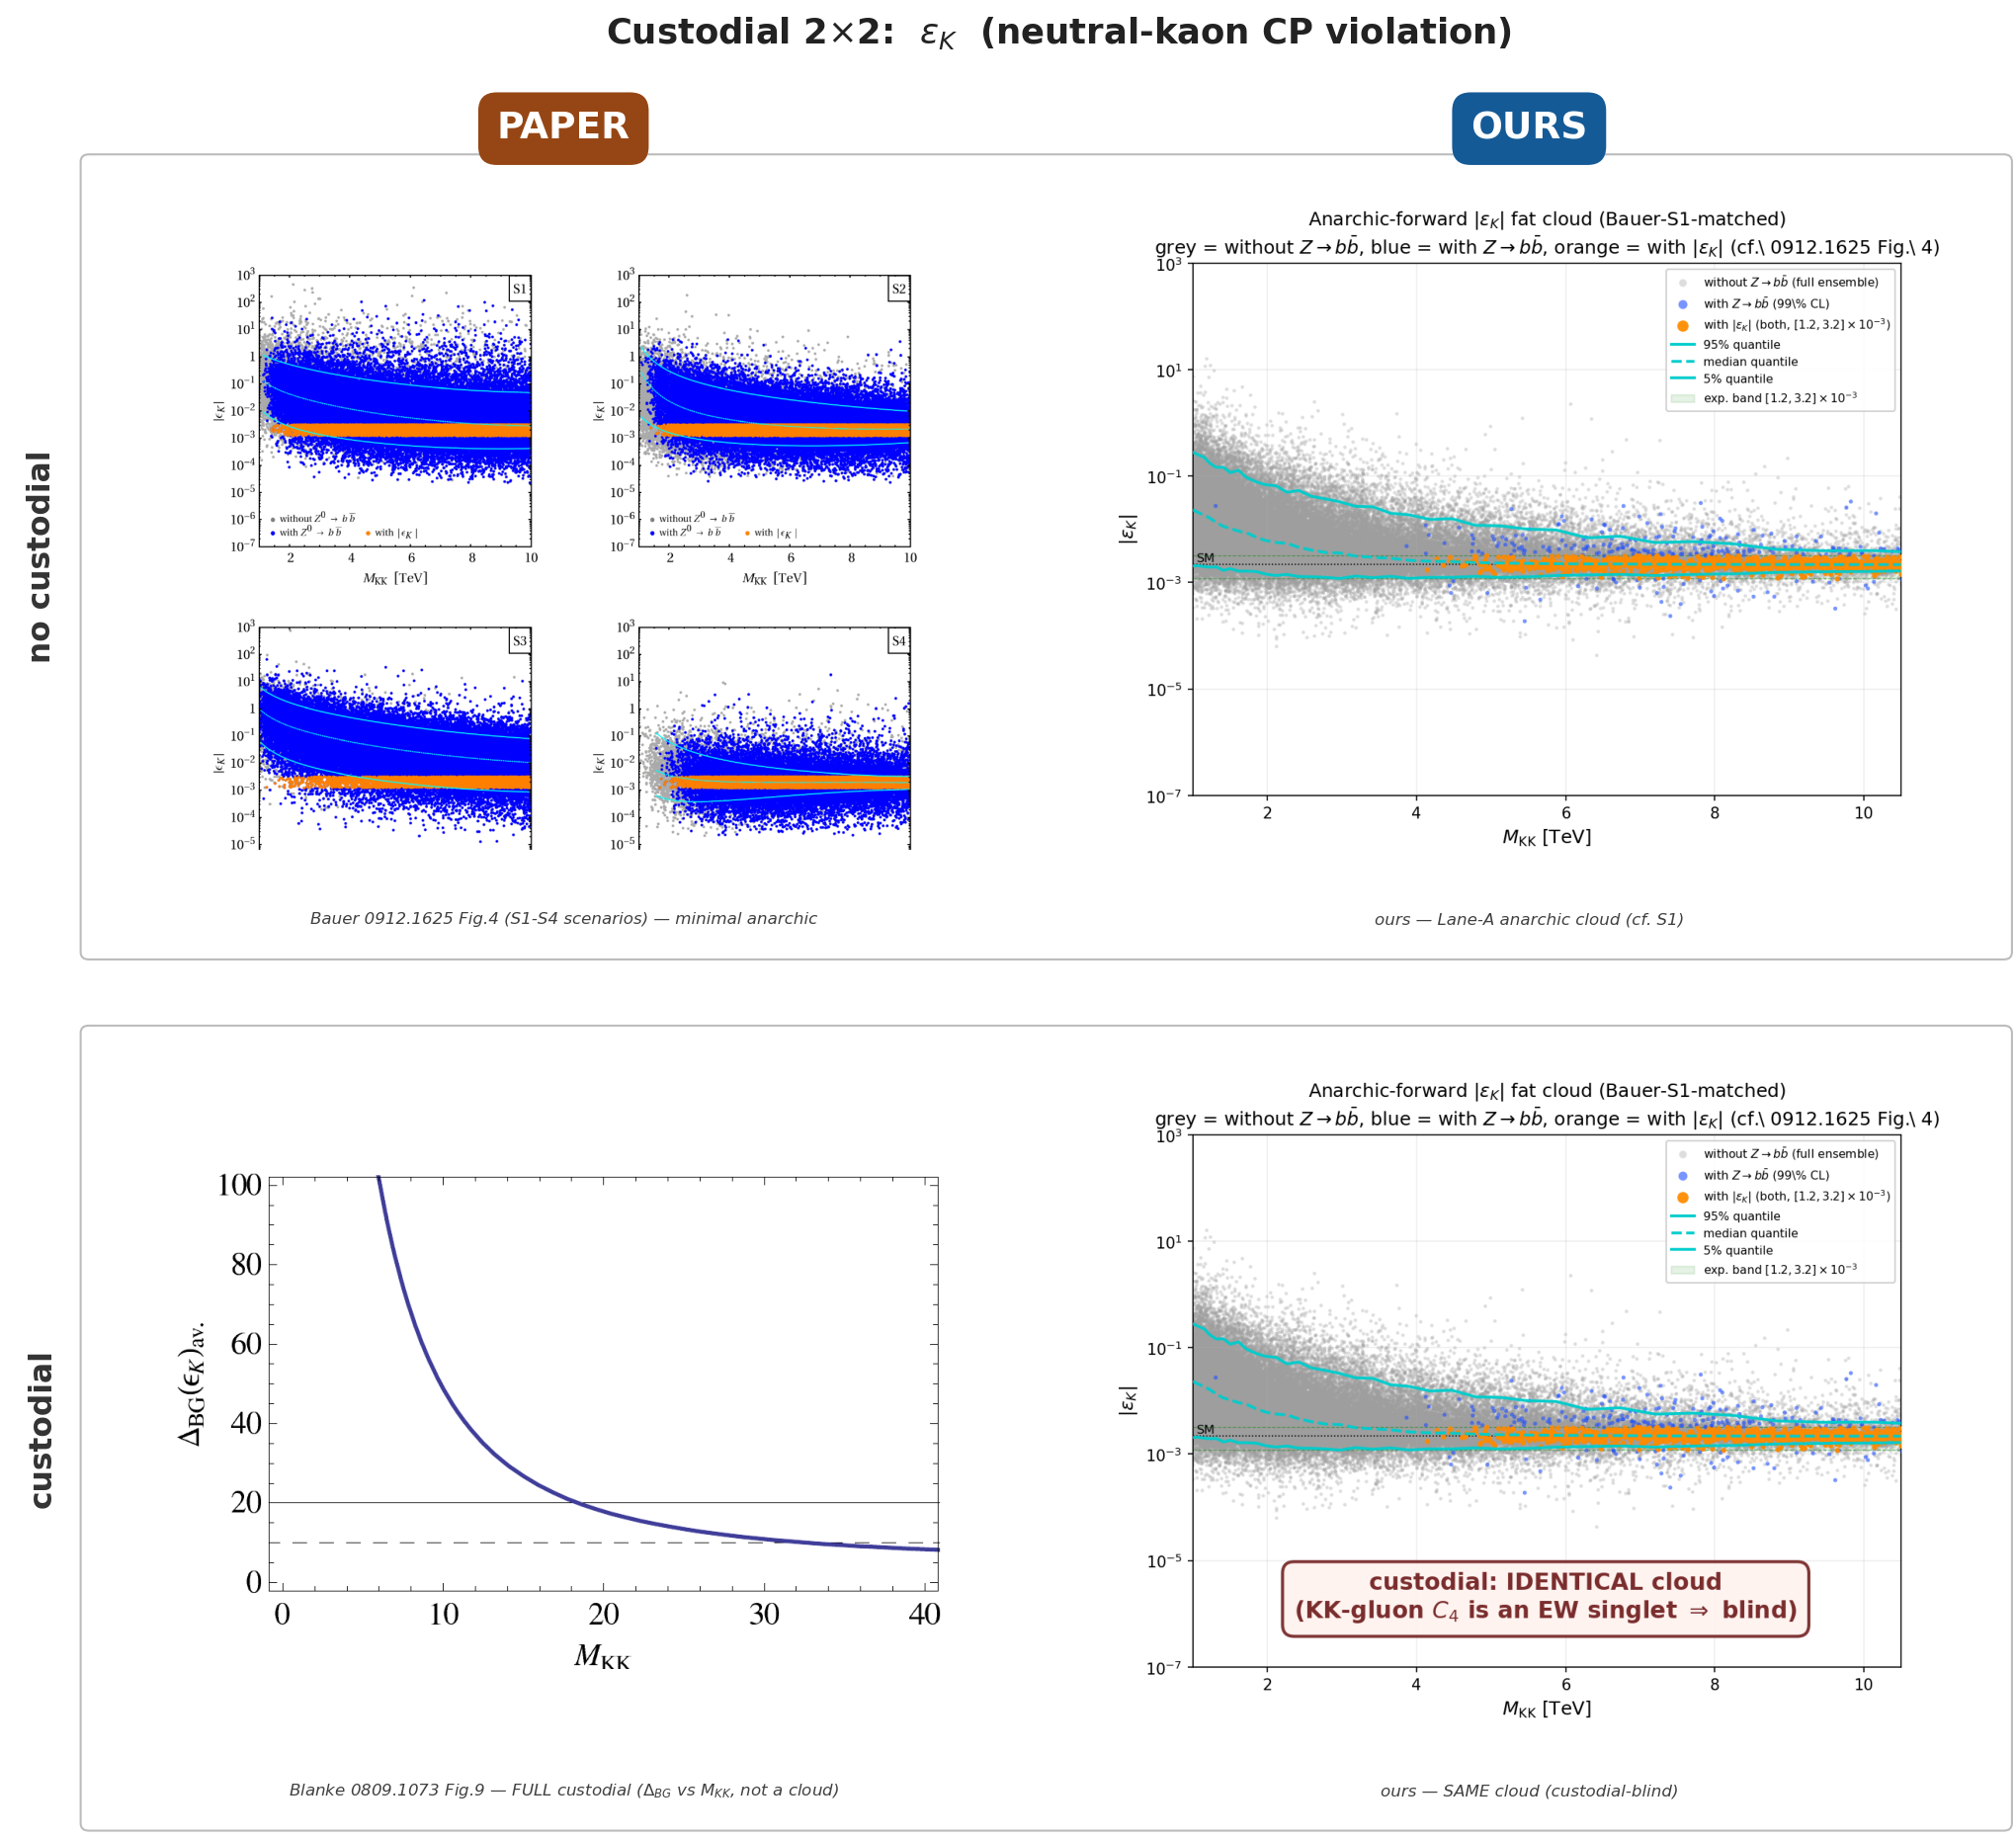
\includegraphics[width=\textwidth]{cmp2x2_epsK.png}
\caption{\textbf{$\varepsilon_K$: custodial is blind to the kaon wall.}
\emph{Top (no custodial):} the minimal anarchic $|\varepsilon_K|$ cloud, Bauer
0912.1625 Fig.~4 (left) and our Lane-A reproduction (right) --- both span
${\sim}6$ decades with the same grey / blue / orange Z$\to b\bar b$ / $|\varepsilon_K|$
layering. \emph{Bottom (custodial):} Blanke 0809.1073 Fig.~9 (left) computes the
$\varepsilon_K$ fine-tuning \textbf{inside the full custodial model} and still
crosses $\Delta_{BG}{<}20$ only at $M_{KK}{\approx}18$~TeV and $\Delta_{BG}{<}10$
at ${\approx}30$~TeV; our custodial panel (right) is the \emph{identical} cloud
plus the annotation, because the KK-gluon $C_4$ operator is an EW singlet that
custodial cannot touch. \textbf{The wall stays at tens of TeV in both the paper
(Blanke, full custodial) and ours.} Floors: ours Lane-A
${\sim}9$--$24$~TeV; literature ${\sim}18$--$33$~TeV (Blanke 18/30, CFW 21/33,
Bauer~II ${\sim}10$, Archer 10--30); custodial moves none of them.}
\end{figure}

\FloatBarrier
\clearpage

% ===================== (2) S,T,U =====================
\section{(2)\quad $S,T,U$ oblique --- custodial pulls $T\to0$}

\begin{figure}[H]
\centering
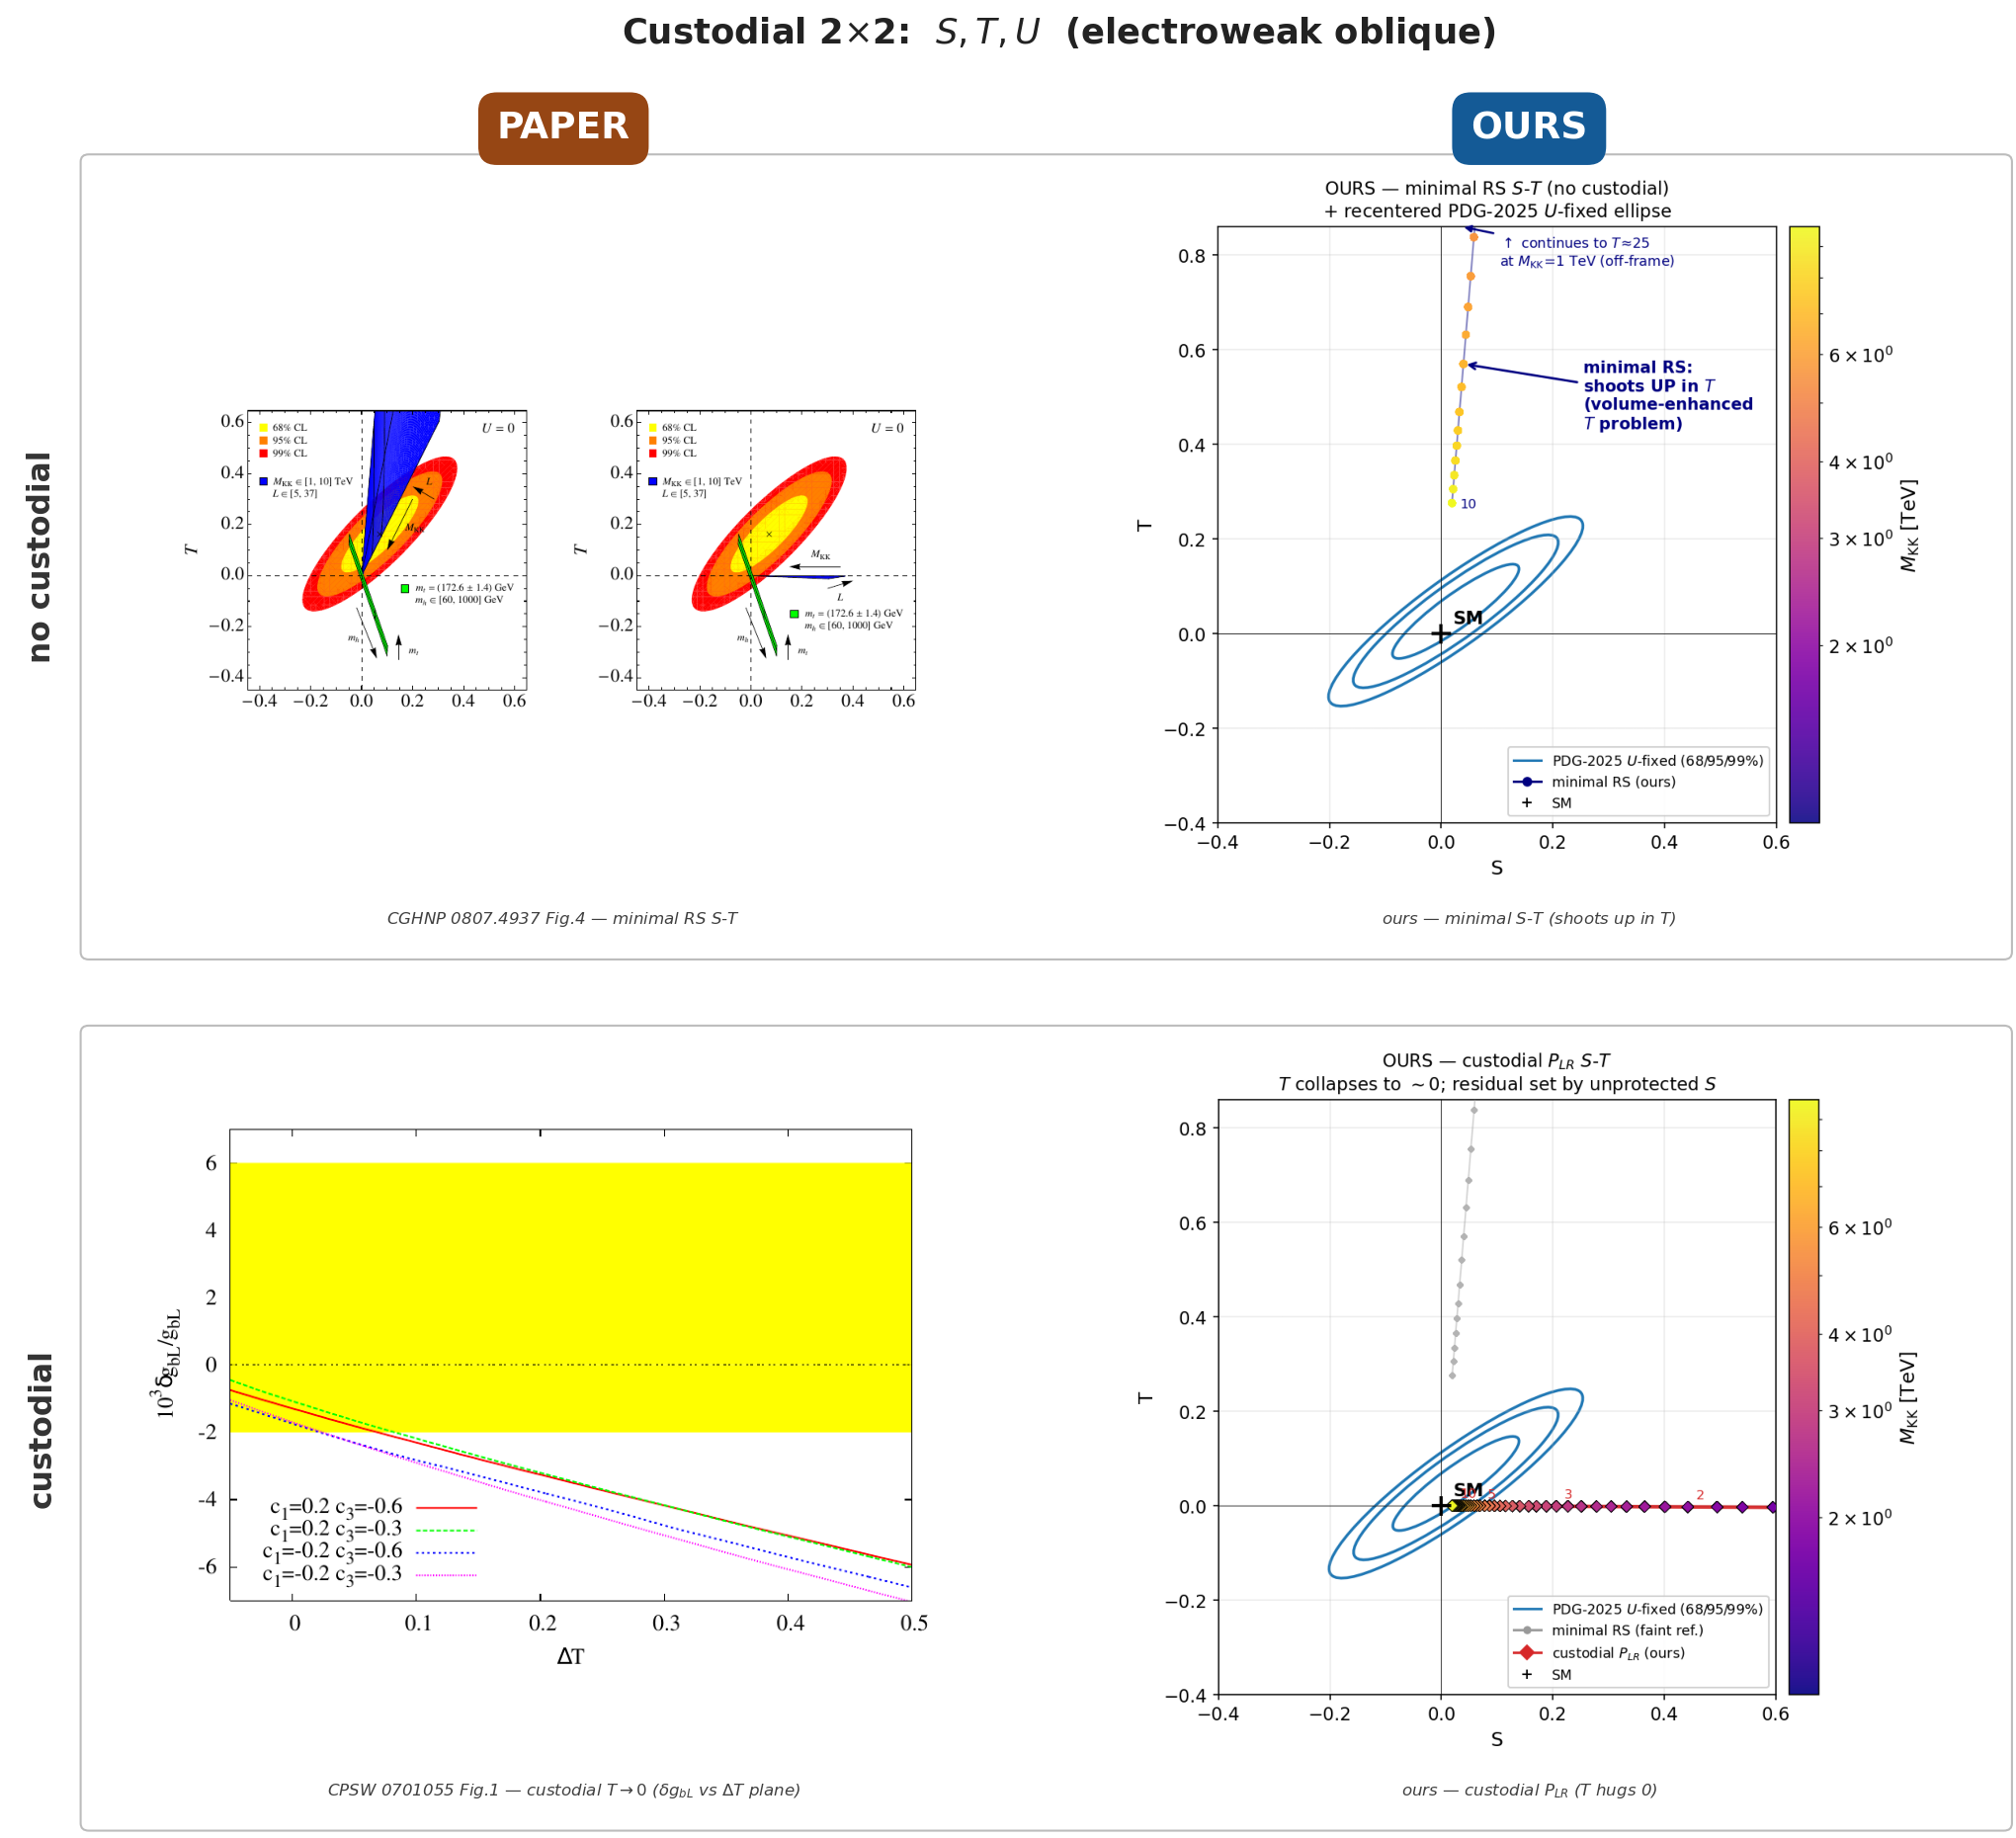
\includegraphics[width=\textwidth]{cmp2x2_STU.png}
\caption{\textbf{$S,T,U$: custodial protects $T$.} \emph{Top (no custodial):}
the minimal RS $S$--$T$ trajectory climbs steeply in $T$ (the volume-enhanced
``RS $T$ problem''), in CGHNP 0807.4937 Fig.~4 (left) and in ours (right, the
points shoot up off the recentered PDG-2025 ellipse). \emph{Bottom (custodial):}
CPSW 0701055 Fig.~1 (left) shows the custodial $\delta g_{bL}$--$\Delta T$
correlation with $\Delta T$ driven back toward $0$; our custodial $P_{LR}$
trajectory (right) hugs the $S$-axis at $T\!\approx\!0$ (minimal $T$ reaches
${\sim}25$ at 1~TeV; custodial $|T|{<}0.01$ everywhere), the ADMS mechanism
($\mathrm{SU(2)}_R$ turns $\Delta T\propto{+}L$ into ${-}1/L$). \textbf{Custodial
relieves the oblique floor in both paper and ours:} our minimal
${\sim}18$--$20$~TeV existence wall $\to$ custodial ${\sim}2$--$3$~TeV
(literature, $S$-limited), with the residual set by the \emph{unprotected} $S$.}
\end{figure}

\FloatBarrier
\clearpage

% ===================== (3) Z->bb =====================
\section{(3)\quad $Z\to b\bar b$ --- custodial collapses onto the SM}

\begin{figure}[H]
\centering
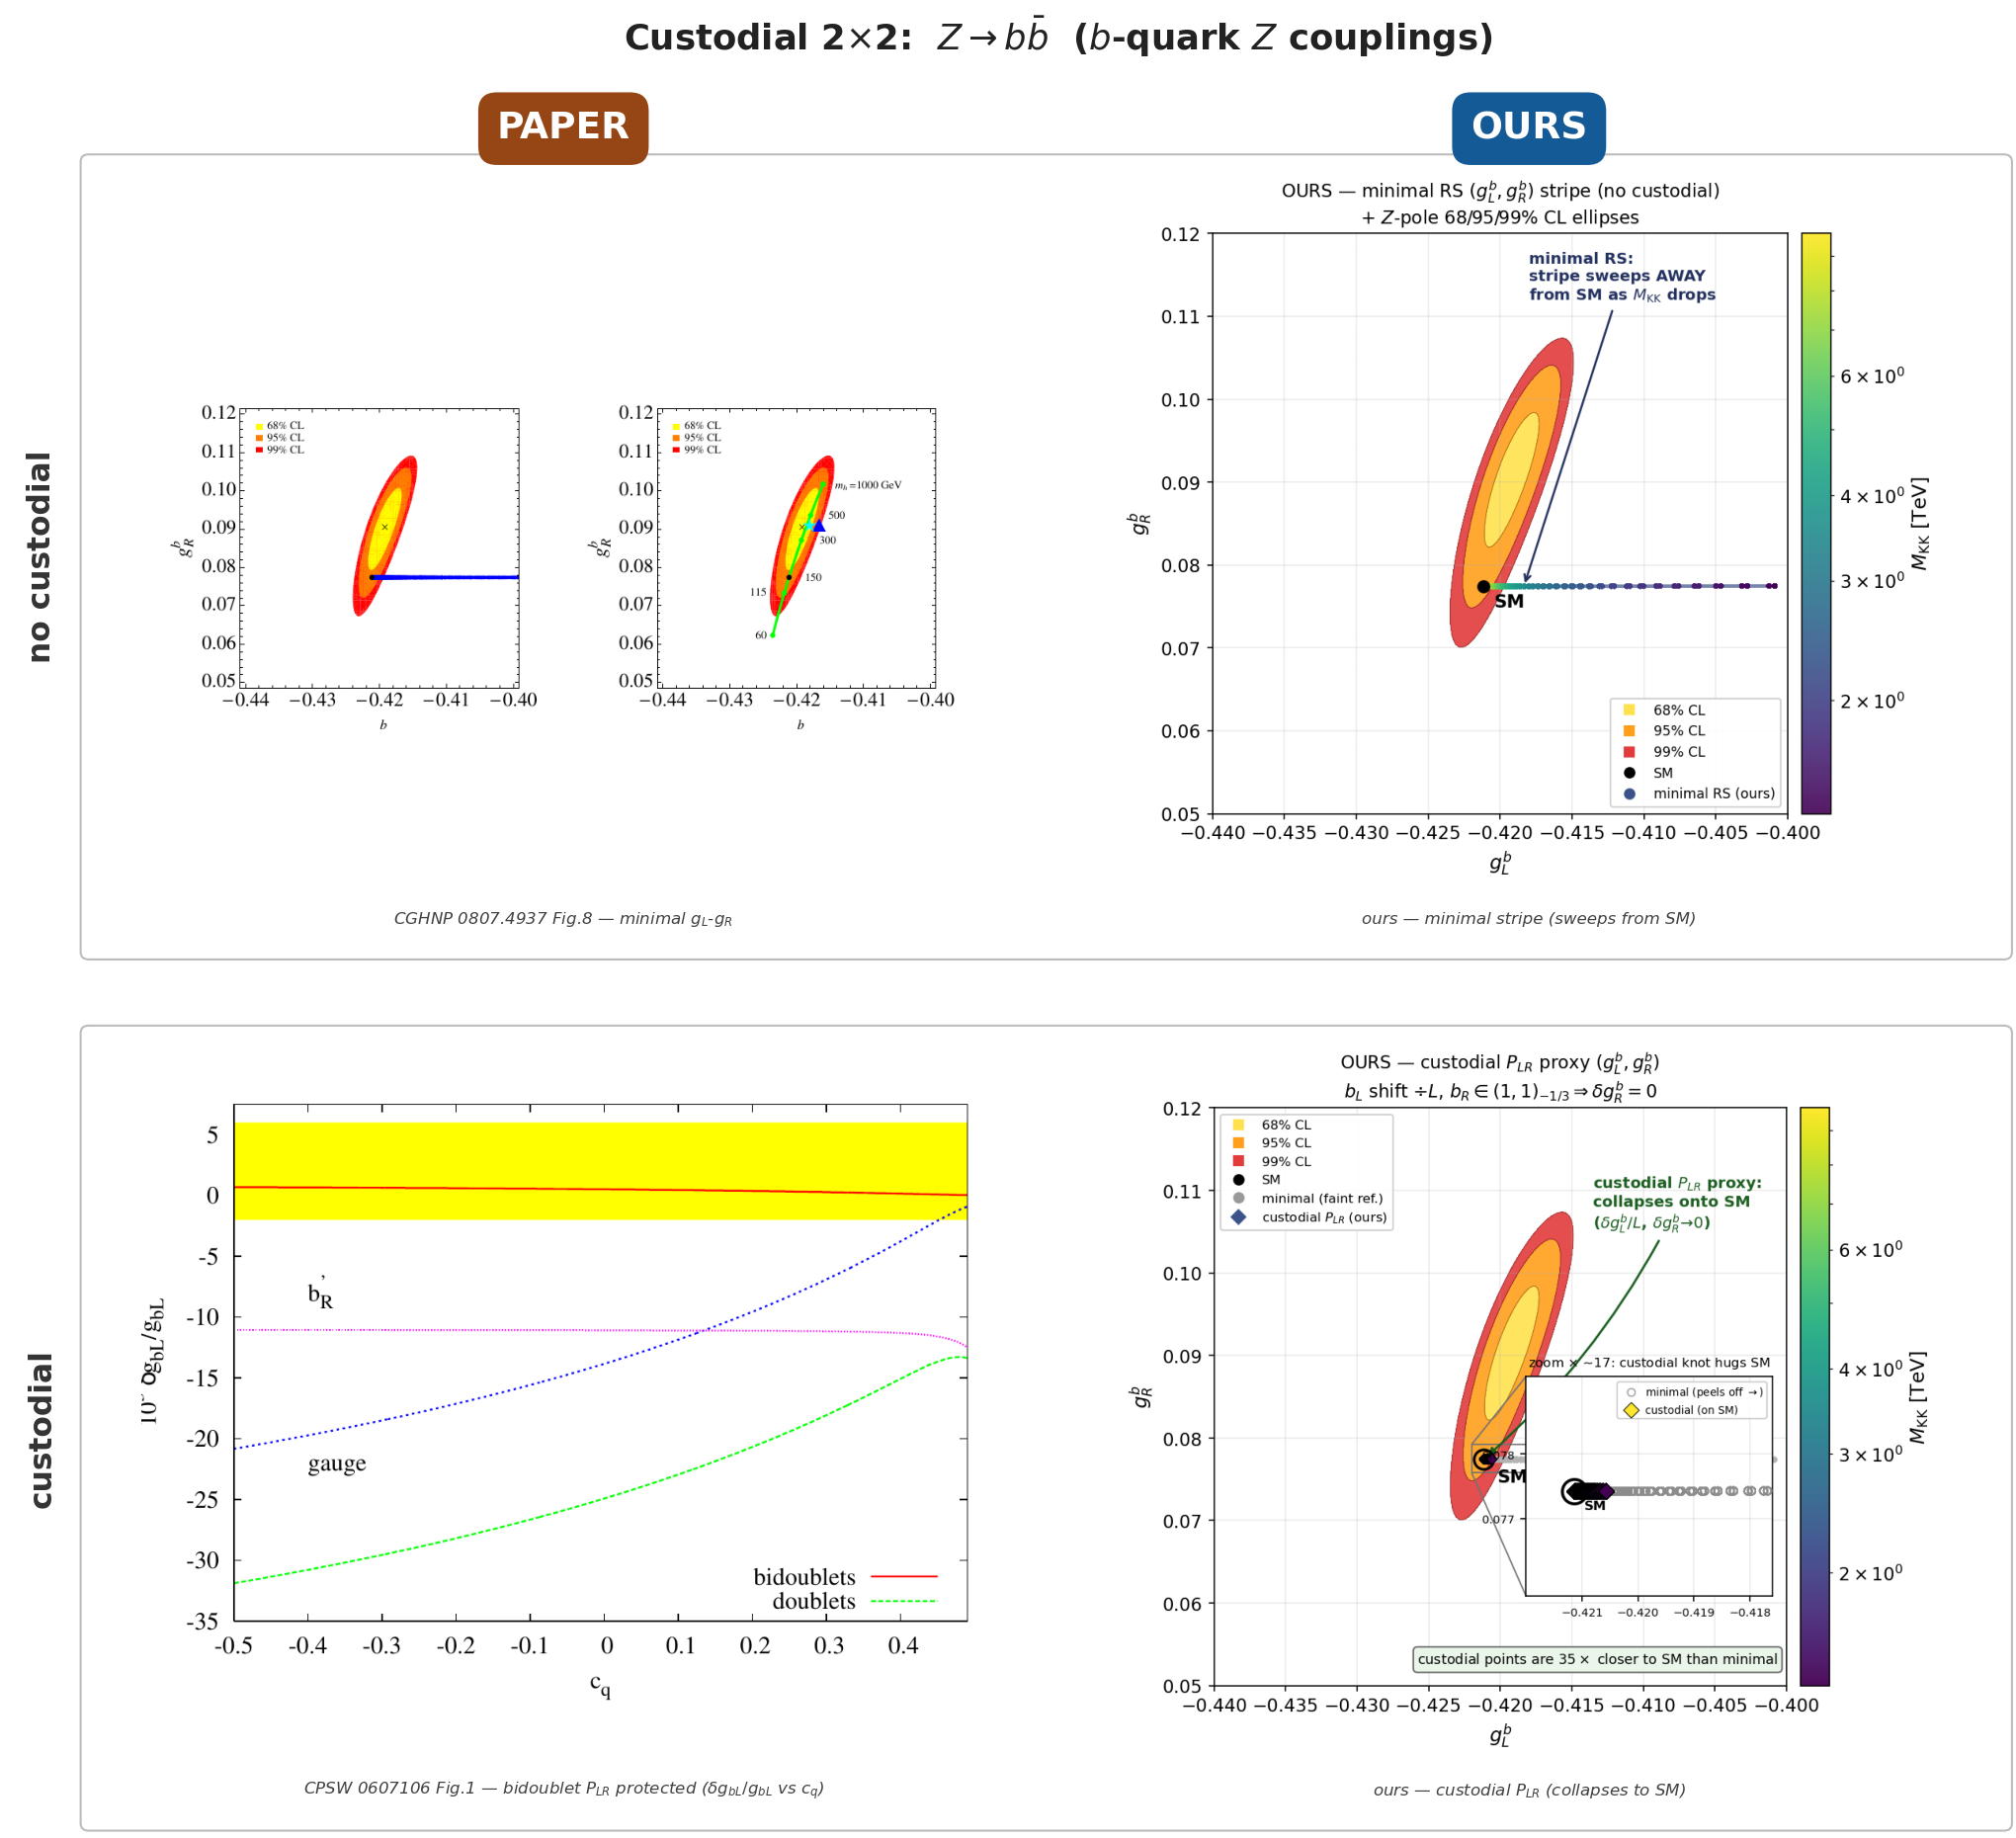
\includegraphics[width=\textwidth]{cmp2x2_Zbb.png}
\caption{\textbf{$Z\to b\bar b$: $P_{LR}$ collapses the $b$ couplings to the SM.}
\emph{Top (no custodial):} the minimal $(g_L^b,g_R^b)$ stripe sweeps away from
the SM as $M_{KK}$ drops, in CGHNP 0807.4937 Fig.~8 (left) and ours (right),
overlaid on the $Z$-pole 68/95/99\% CL ellipses. \emph{Bottom (custodial):} CPSW
0607106 Fig.~1 (left) --- the \textbf{bidoublet} embedding (red) sits inside the
allowed band because $P_{LR}$ with $b_L\in(2,2)_{2/3}$ zeroes $\delta g_L^b$ at
tree level, while the unprotected ``gauge'' / ``doublets'' curves run far below;
our custodial $P_{LR}$ proxy (right) collapses onto the SM point ($\delta g_L^b$
suppressed by $1/L$, $\delta g_R^b\!\to\!0$ for $b_R\in(1,1)_{-1/3}$), landing
${\sim}35\times$ closer to the SM than the minimal stripe. \textbf{Custodial
protects $Z b_L\bar b_L$ at tree level in both paper and ours} (top-partner loops
partially re-introduce it; see \texttt{custodial\_comparison.tex}). Floor: our
minimal $Z\to b\bar b$ bites only to ${\sim}5$~TeV (post-B1-fix; the old
$25$--$30$~TeV was a sign-bug).}
\end{figure}

\FloatBarrier
\clearpage

% ===================== CLOSING =====================
\section{Bottom line}

\headlinebox{%
\begin{itemize}\setlength{\itemsep}{0.35em}\leftskip-0.6em
\item \textbf{Custodial is an EW cure, not a flavor cure.} It pulls $T\to0$ and
collapses the $Z\,b\bar b$ shifts onto the SM, but leaves the $\varepsilon_K$
wall flat at tens of TeV --- in the literature (Blanke's full custodial
$\Delta F{=}2$) and in ours.
\item \textbf{The EW floors drop, the flavor wall does not.} $S,T,U$:
${\sim}18$--$20$~TeV $\to{\sim}2$--$3$~TeV ($S$-limited). $Z\to b\bar b$:
tree-protected. $\varepsilon_K$: unchanged at tens of TeV; only flavor
\emph{alignment} (lane C) moves it to ${\sim}2$~TeV.
\item \textbf{These plots show the leading physics only.} The OURS custodial
panels use a leading-order tree EW proxy (custodial $T$, $P_{LR}$ $Z b_L\bar b_L$
protection); the subleading custodial phenomenology is the deferred full build,
scoped in \texttt{custodial\_comparison.tex}.
\end{itemize}}

\end{document}
